\chapter{Déroulement du stage}
\clearpage


\section{Prise de fonction}
J'avais commencé officiellement le stage le 1er Août 2024 dans les locaux de la Société Sirius Digital. J'ai bien été accueillis dans le cadre du stage. 
Le stage commence tous les jours de 7h à 12h et de 14h à 17h de lundi à Vendredi marquée par une pose de 12h à 14h ou l'on es libre de ses actions.
L'entreprise m'a été présenté par un des membres de l'équipe déjà en place suivit d'une explication de DG qui, avait bien compris ma mission au sein de l'entreprise et m'expliquer les choses étapes par étapes pour l'avancement du projet.


\begin{itemize}
    \item Découvert l'environnement de travail et les outils utilisés.
    \item Échangé avec les membres de l'équipe et le DG pour mieux comprendre les besoins et le cadre du stage.

\end{itemize}
\section{Tâches effectuées}
Pendant ce stage, j'ai eu à effectuer plusieurs tâches notamment
\begin{itemize}
    \item Modélisation des différents diagrammes
    \item Développement Web
    \item Rédaction du support technique
    \item Rédaction du manuel d'utilisation    
\end{itemize} 


\subsubsection{Illustration}
\begin{figure}[H]
    \centering
    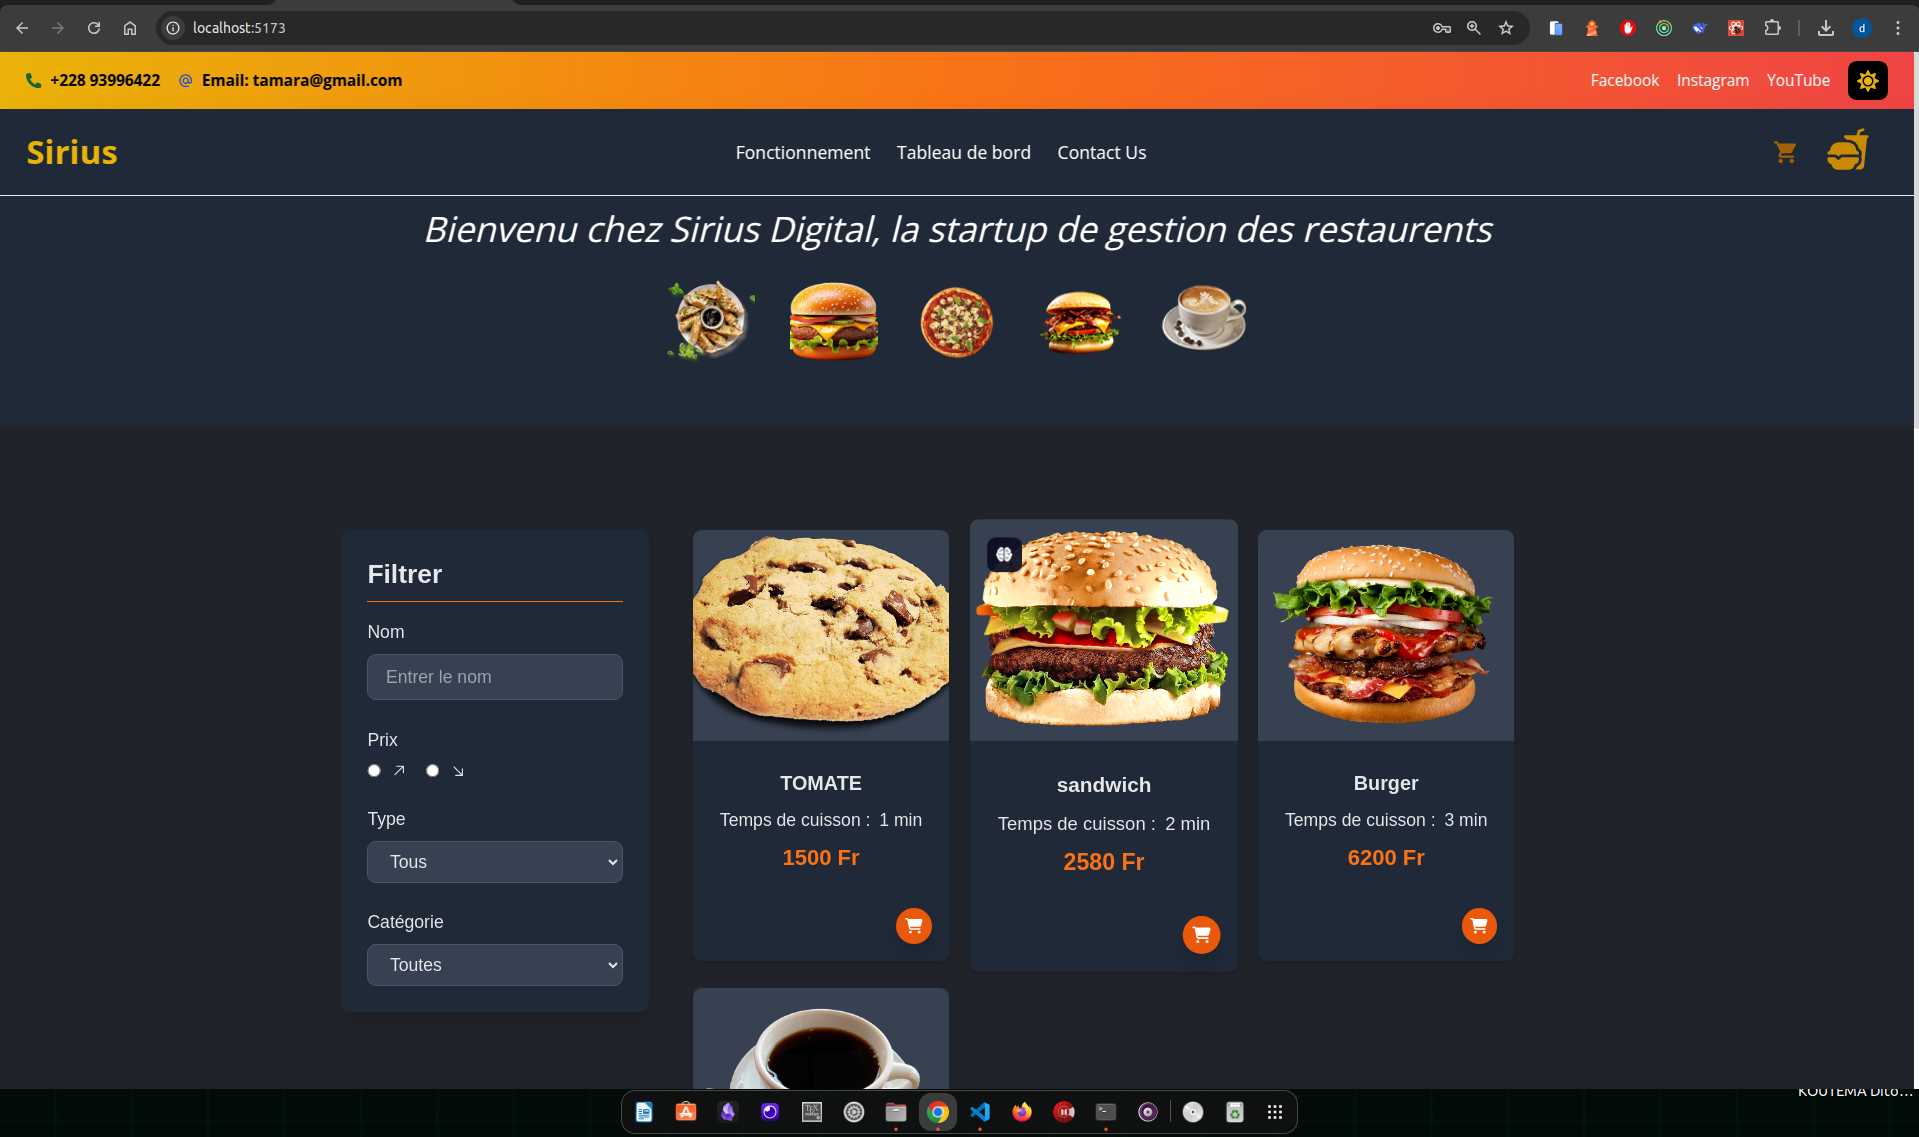
\includegraphics[width=0.8\textwidth]{images/passe/home.png}
    \caption{Page d'accueil de la \ac{PASSE}}
    \label{fig:page-accueil_pass}
\end{figure}

\begin{figure}[H]
    \centering
    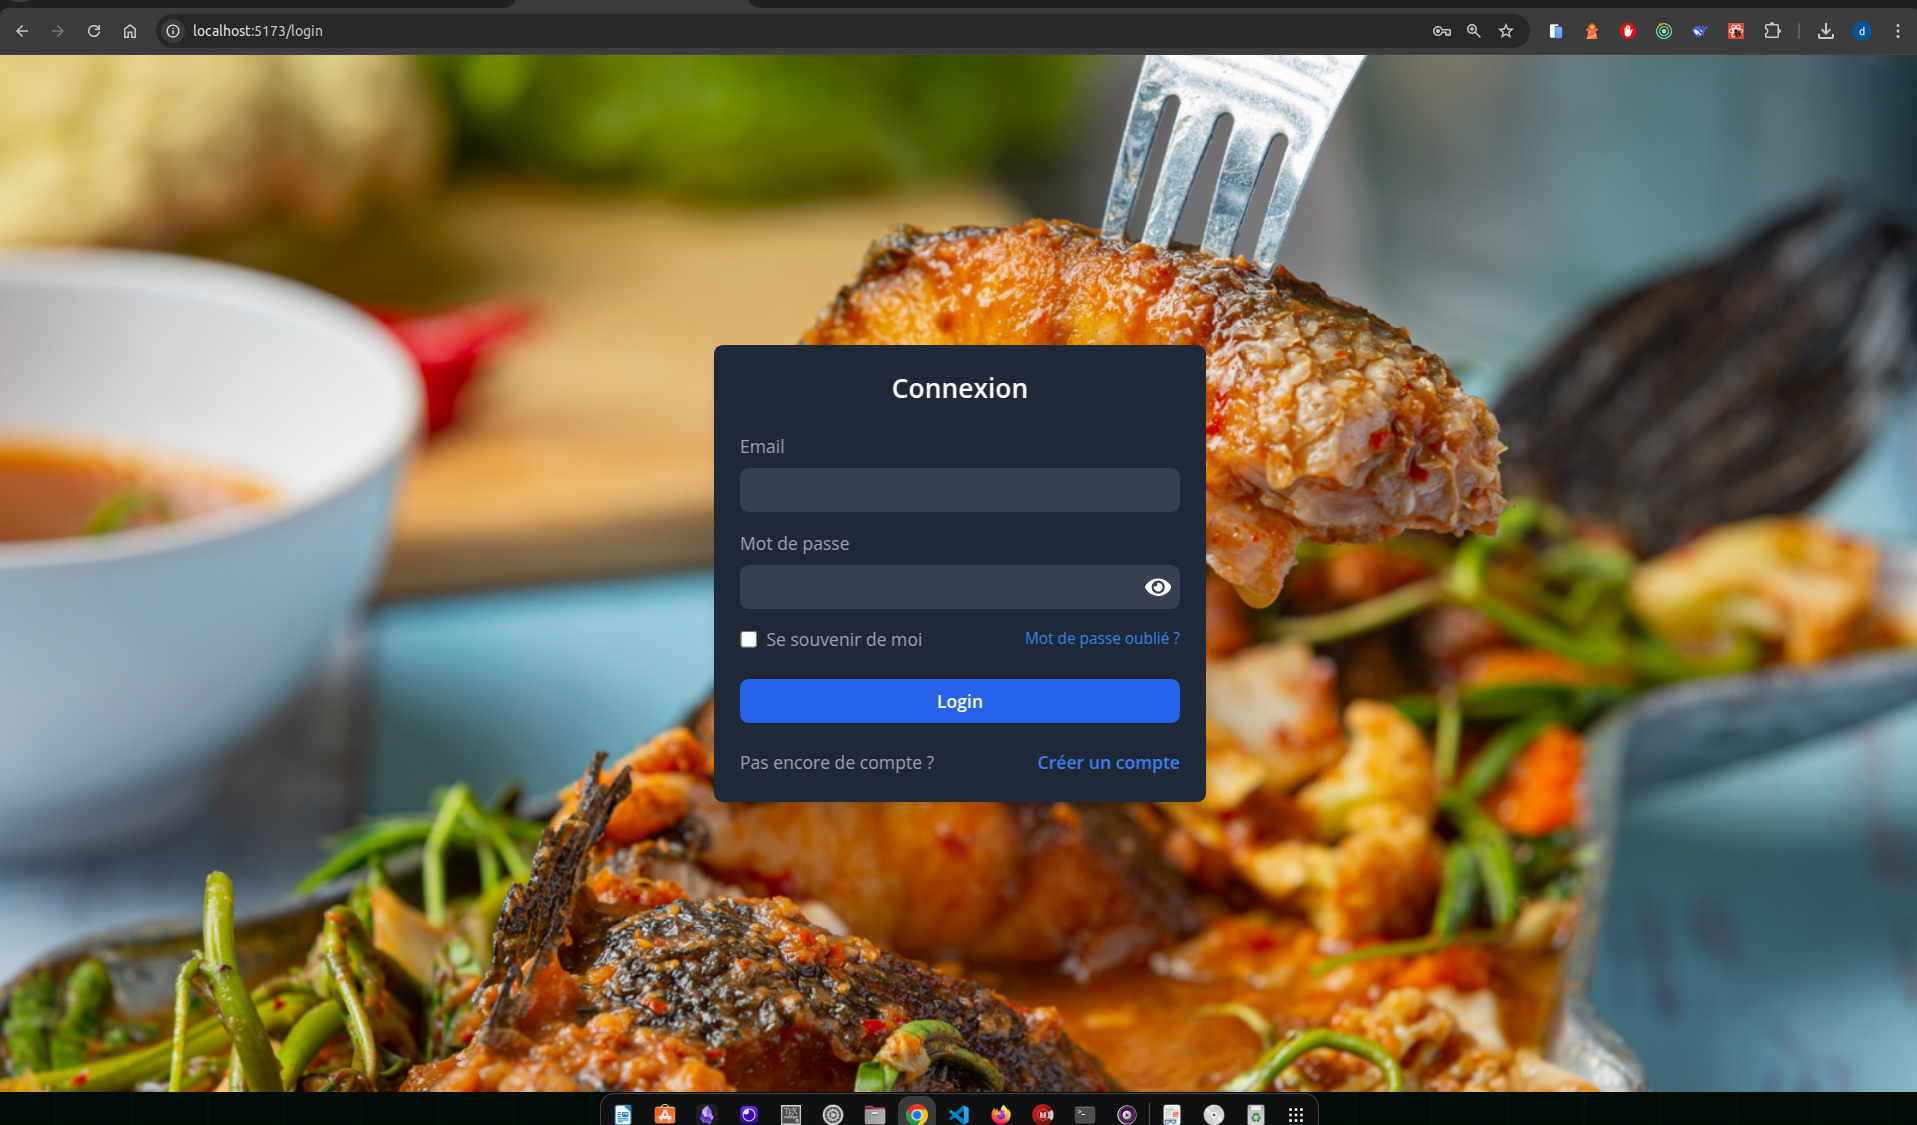
\includegraphics[width=0.8\textwidth]{images/passe/login.png}
    \caption{Interface de connexion de la \ac{PASSE}}
    \label{fig:interface-login_pass}
\end{figure}

\begin{figure}[H]
    \centering
    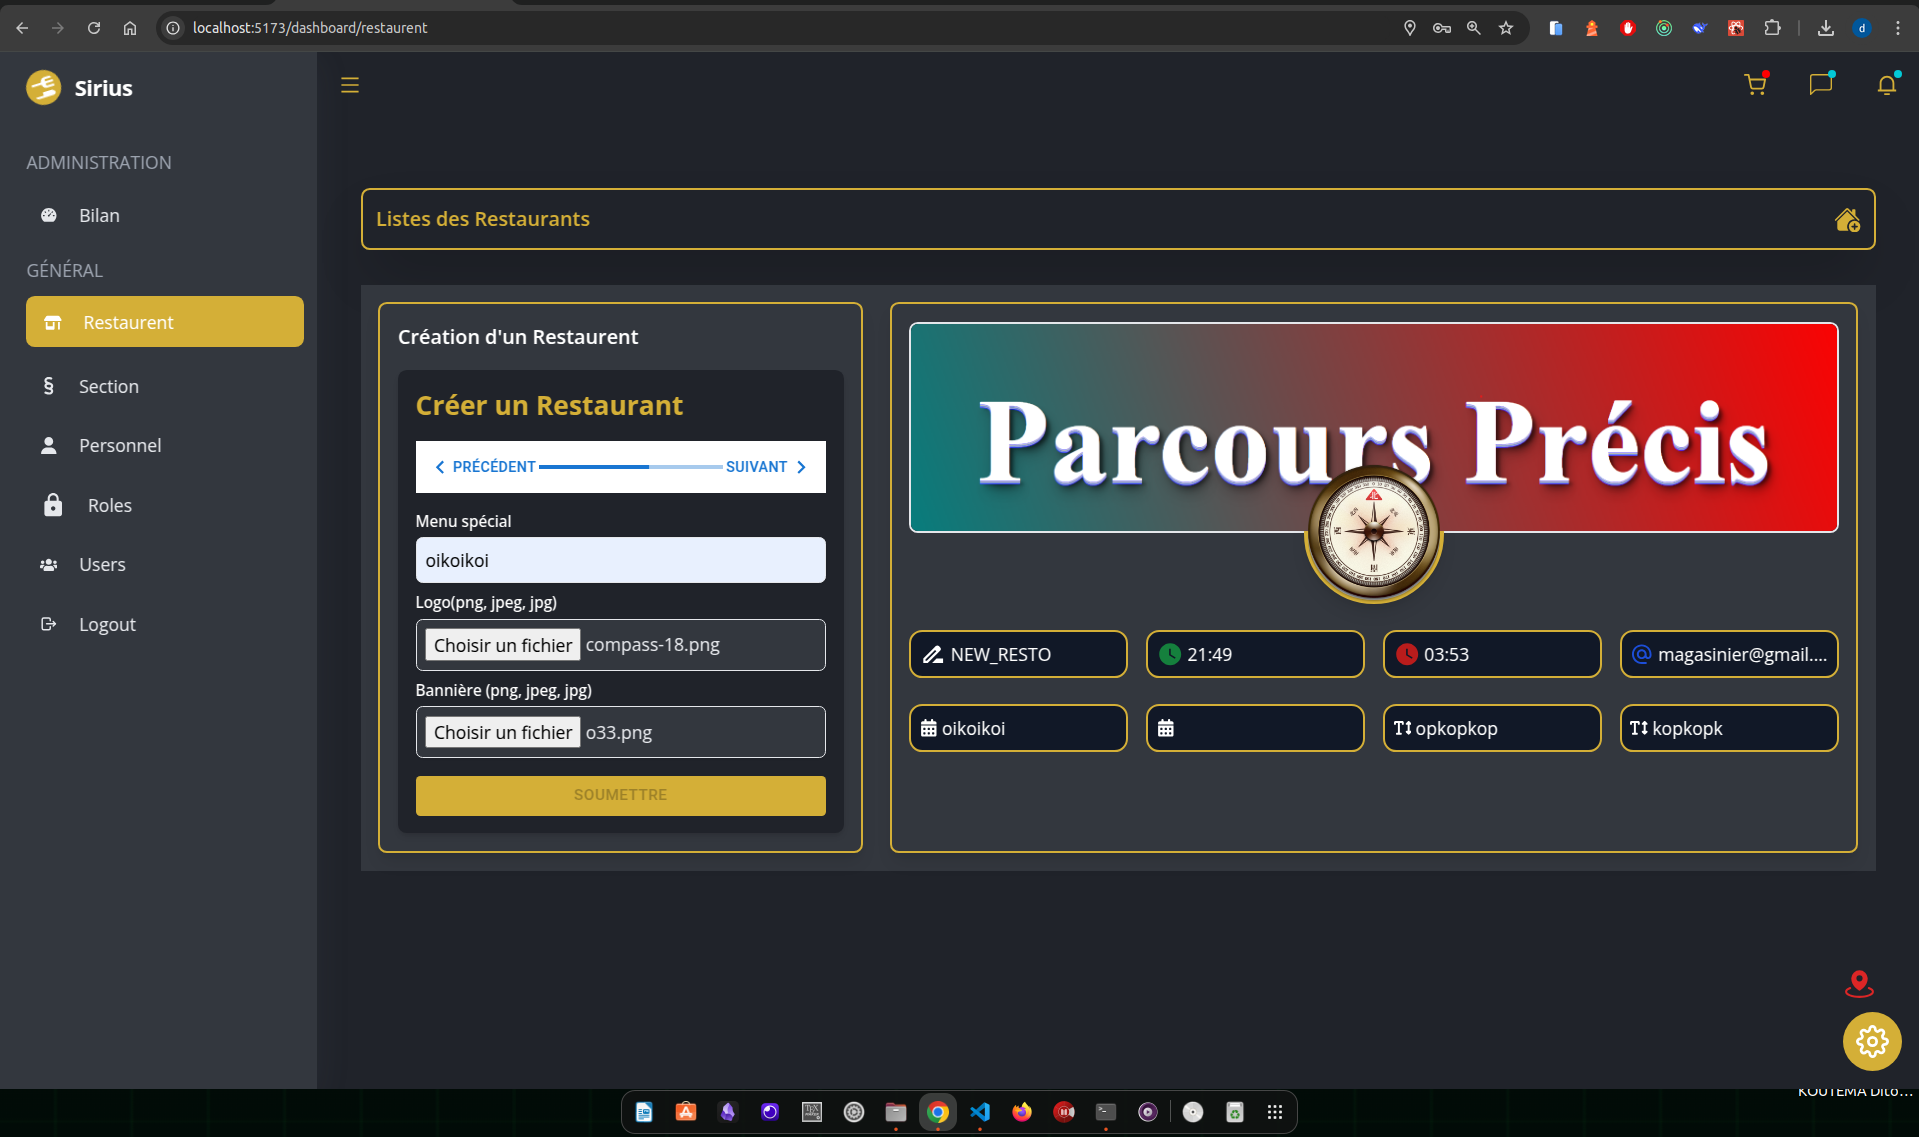
\includegraphics[width=0.8\textwidth]{images/passe/dash.png}
    \caption{Interface de connexion de la \ac{PASSE}}
    \label{fig:interface-login_pass}
\end{figure}








\subsection{Assistance technique générale}
En complément des missions spécifiques, un support technique global a été assuré au sein de l’organisation :
\begin{itemize}
    \item Dépannage et maintenance des outils informatiques utilisés par le personnel.
    \item Configuration et optimisation des postes de travail selon les besoins des employés.
    \item Sensibilisation aux bonnes pratiques pour garantir la pérennité des équipements et la sécurité des données.
\end{itemize}
\section{Remarques et suggestions}
\section{Bilan et conclusion}
Cette expérience a permis de mieux appréhender les enjeux liés à la gestion d’un service informatique, alliant assistance aux utilisateurs, maintenance technique et développement d’outils numériques.

\clearpage
